\documentclass[13pt, a4paper,headinclude, 
footinclude, 
plainfootsepline]{scrreprt} % Defines the font size and the paper format

\usepackage[english]{babel}
\usepackage[utf8]{inputenc}
\usepackage{textcomp}
\usepackage{amsmath, amssymb, amsfonts} % Standard AMS packages
\usepackage{amsthm}           % For theorem environments
\usepackage{geometry}         % Customize page geometry
\usepackage{setspace}         % To set line spacing
\usepackage{graphicx}
\usepackage[automark,headsepline,footsepline]{scrpage2}
\usepackage{pdfpages}
\usepackage{color}
\usepackage{listings}
\usepackage{float}
\usepackage{pgfplots,pgfplotstable}
\usepackage{caption}
\usepackage{setspace}

%--------------------------------------------------------------------
%--- Configure Listing Design
%--------------------------------------------------------------------
\definecolor{pblue}{rgb}{0.13,0.13,1}
\definecolor{pgreen}{rgb}{0,0.5,0}
\definecolor{pred}{rgb}{0.9,0,0}
\definecolor{pgrey}{rgb}{0.46,0.45,0.48}

\lstdefinestyle{lstStyle}{
	language=java,
	numbers=left,
	stepnumber=1,
	numbersep=10pt,
	tabsize=4,
	showspaces=false,
	showstringspaces=false
}

\lstset{
	basicstyle=\tiny,
	style=lstStyle,
	frame=tb,
	language=Java,
	showspaces=false,
	showtabs=false,
	breaklines=true,
	columns=fullflexible,
	showstringspaces=false,
	breakatwhitespace=true,
	basicstyle=\ttfamily,
	tabsize=3
}
%--------------------------------------------------------------------
%--- Title, author, date
%--------------------------------------------------------------------

\newcommand{\theuniversity}{Brunel University London}
\newcommand{\thecollege}{College of Engineering, Design and Physical Sciences}
\newcommand{\thedepartment}{Department of Engineering and Design}
\newcommand{\thecoursetitle}{Assignment \\ Workshop EE5614}
\newcommand{\thestudent}{Tobias \textsc{Schwarz}}
\newcommand{\thestudentid}{1744864}
\newcommand{\thestudenttwo}{Stephan \textsc{Dittmann}}
\newcommand{\thestudentidtwo}{1744874}
\newcommand{\thestudentthree}{Roland \textsc{Flat}}
\newcommand{\thestudentidthree}{1744872}
\newcommand{\thesupervisor}{Satikidis Dionysis}
\newcommand{\theyear}{2018}
\newcommand{\thetitle}{Embedded Systems}
\newcommand{\code}[1]{\texttt{#1}}


%--------------------------------------------------------------------
%--- Global page geometry and layout
%--------------------------------------------------------------------

% Define the page margins
\geometry{
	left=40mm,
	right=25mm,
	bindingoffset=0mm, 
	top=25mm,
	bottom=25mm,
	headsep=15mm
}
\setlength\parindent{0pt}
\addtokomafont{disposition}{\rmfamily}
\pagestyle{scrheadings}
\renewcommand*{\chapterheadstartvskip}{\vspace*{-0.5cm}}
\renewcommand*{\chapterheadendvskip}{\vspace{7.5mm}}
\renewcommand{\chapterpagestyle}{scrheadings}
% Kopf- und Fußzeile auch auf Kapitelanfangsseiten
\clearscrheadfoot
% Schriftform der Kopfzeile
\renewcommand{\headfont}{\normalfont}
% Kopfzeile
\ihead{Project Control and Management}
\chead{}
\ohead{
\includegraphics[scale=0.15]{BasePictures/Brunel_University_Logo.png}}
%Fußzeile
\ifoot[Tobias Schwarz]{Tobias Schwarz, Stephan Dittmann, Roland Flat}
\ofoot[\pagemark]{\pagemark}
\setheadsepline{.5pt}
\setfootsepline{.5pt}
%---------------------------------------------------------------------
%--- Theorem environments
%---------------------------------------------------------------------

% Theorem counter is subordinate to chapter; all theorem-like
% environments are using the same counter
\theoremstyle{plain}
\newtheorem{theorem}{Theorem}[chapter]          
\newtheorem{lemma}[theorem]{Lemma}
\newtheorem{proposition}[theorem]{Proposition}
\newtheorem{corollary}[theorem]{Corollary}

\theoremstyle{definition}
\newtheorem{definition}[theorem]{Definition}
\newtheorem{remark}[theorem]{Remark}

%---------------------------------------------------------------------
%--- Bibliography
%---------------------------------------------------------------------

\usepackage[style=numeric, minnames=3,
            doi=false, url=false, isbn=false,
            firstinits=true,
            sortcites=true,
            backend=bibtex]{biblatex}

\addbibresource{bibliography.bib}

%---------------------------------------------------------------------
%--- Document begins here
%---------------------------------------------------------------------

\begin{document}
	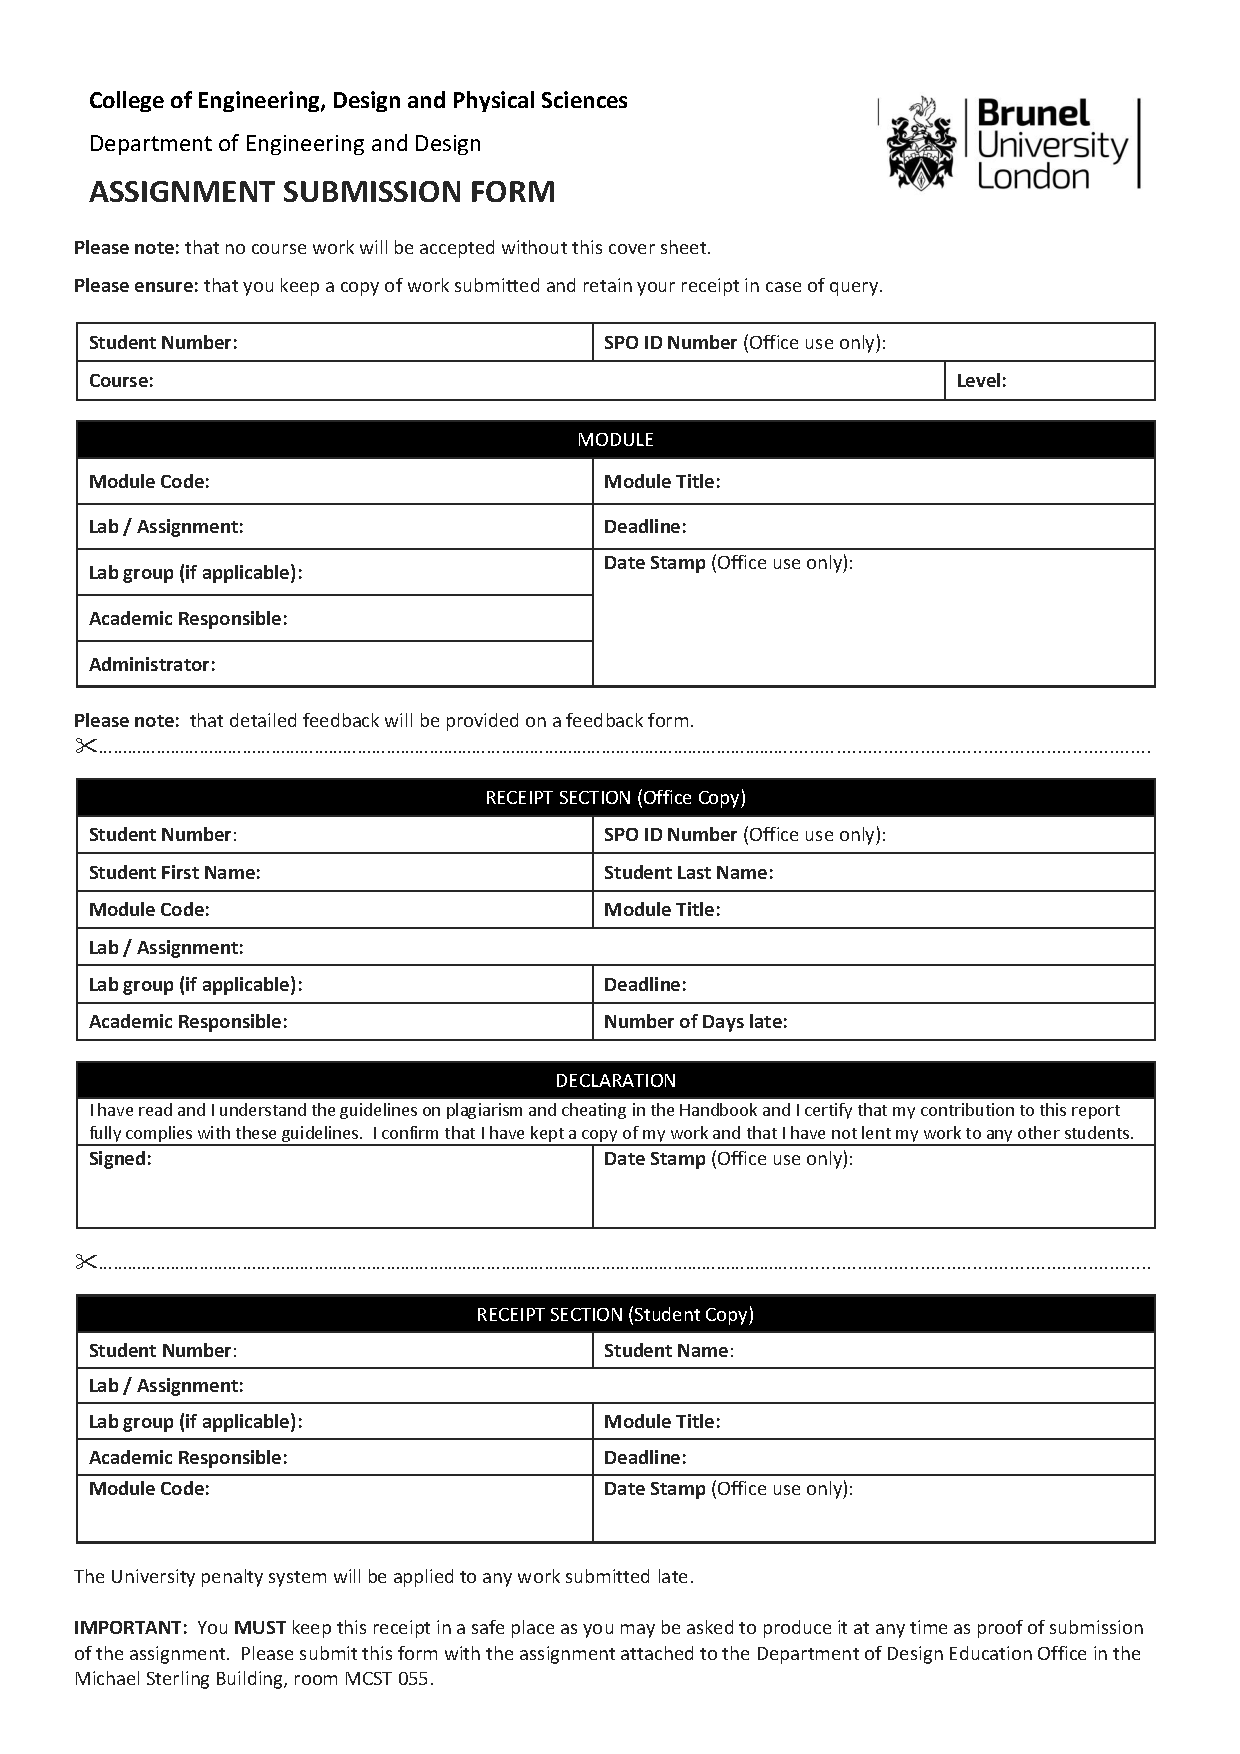
\includepdf{BasePictures/SubmissionForm.pdf}
	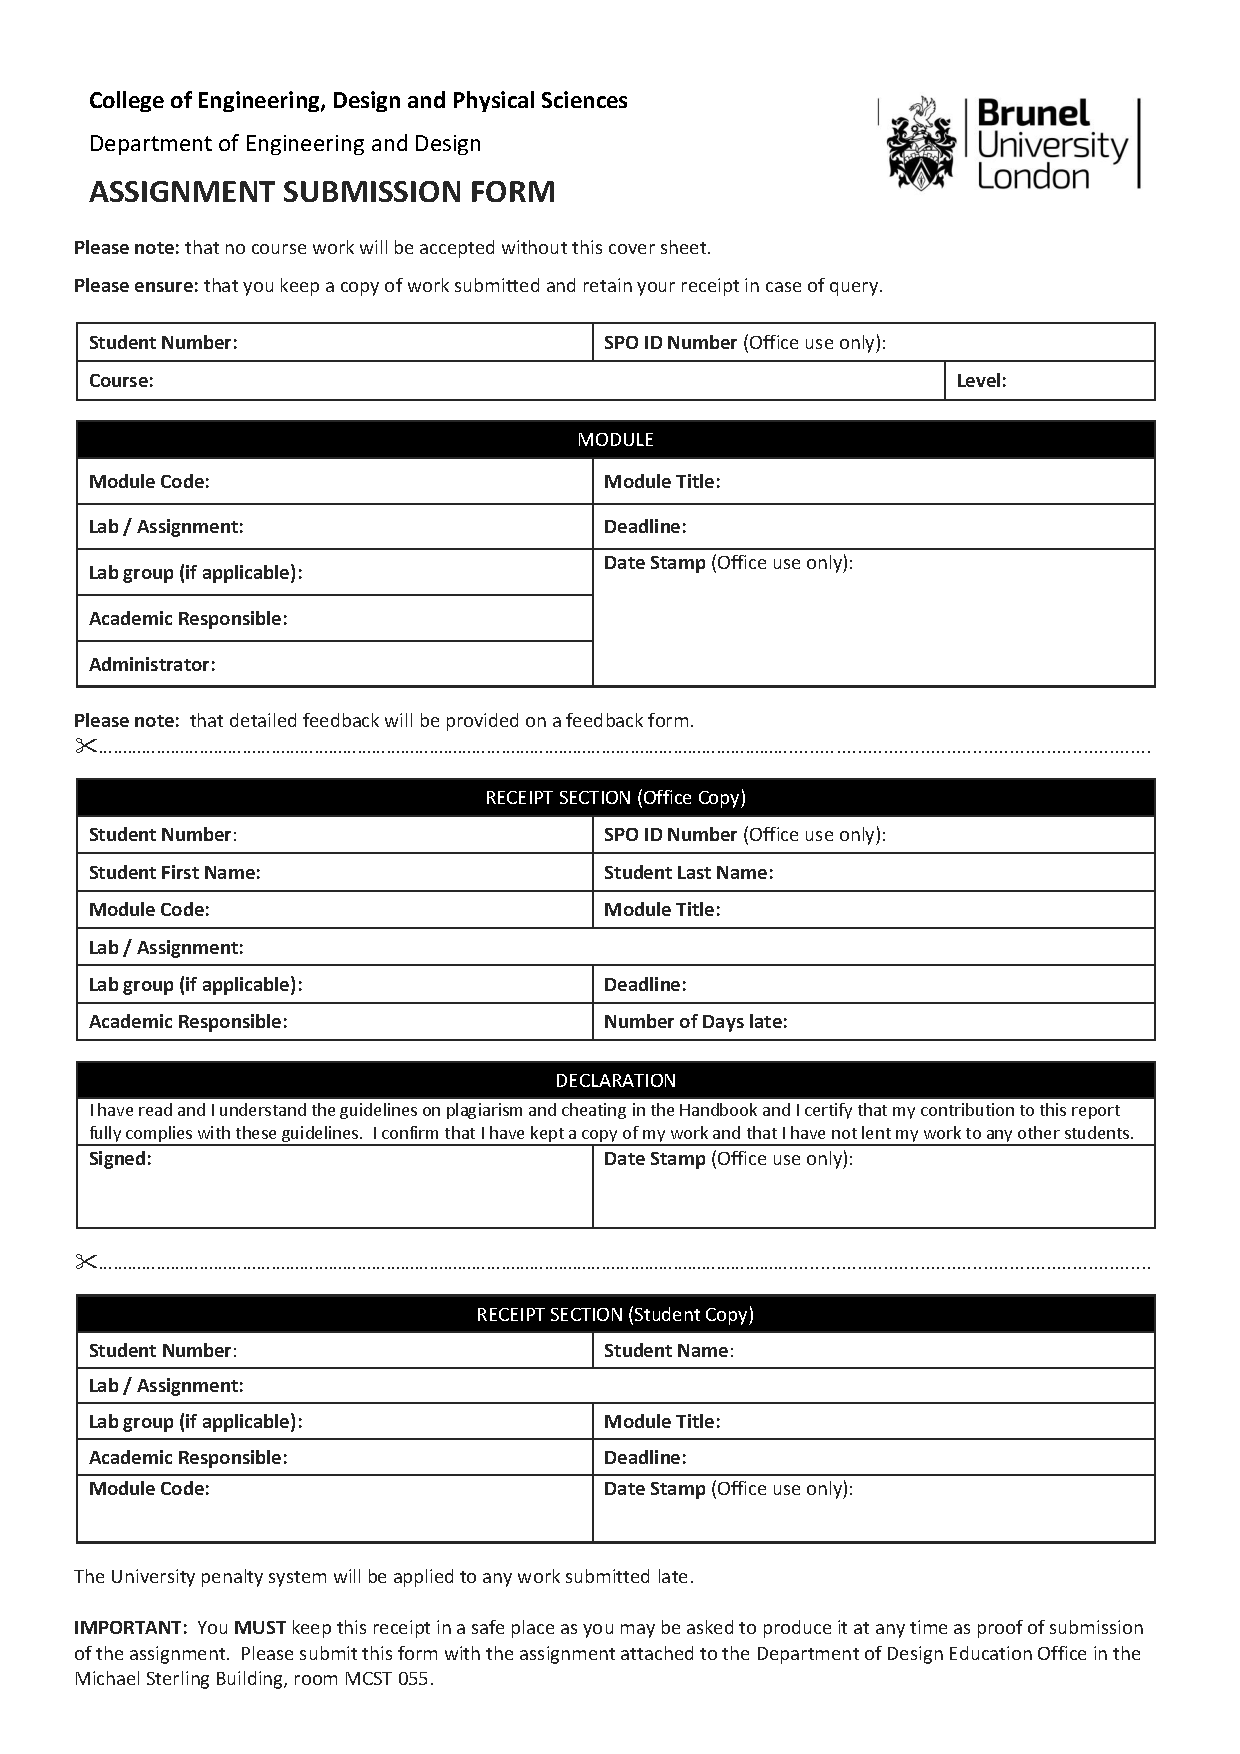
\includepdf{BasePictures/SubmissionForm.pdf}
	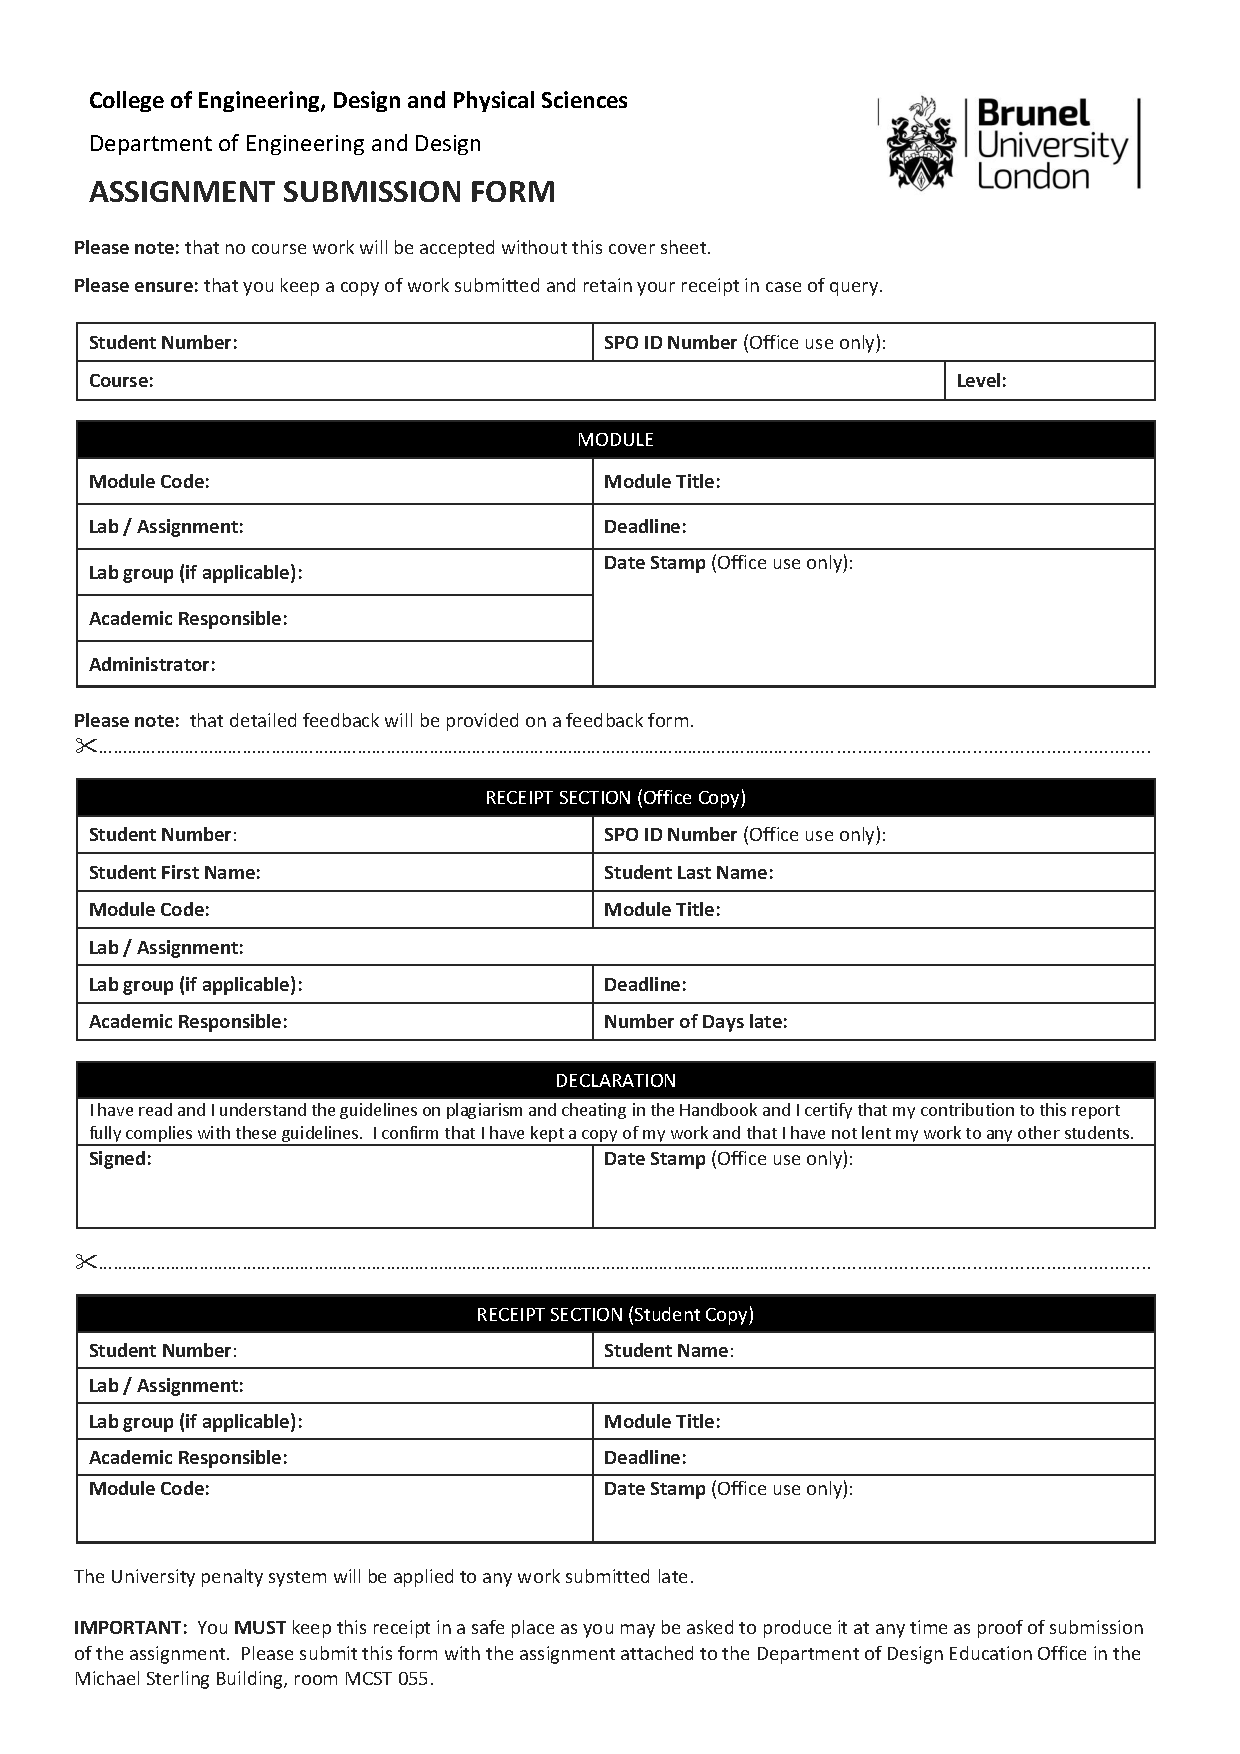
\includepdf{BasePictures/SubmissionForm.pdf}
\onehalfspacing

%---------------------------------------------------------------------
%--- Title page
%---------------------------------------------------------------------

\begin{titlepage}
	\center
	
	% Name of university, college, department and degree
	\textsc{\LARGE \theuniversity} \\[1.5cm] 
	\textsc{\large 
		\thecollege \\
		\thedepartment} \\[1.5cm]
	\textsc{\Large \thecoursetitle} \\[3.0cm]
	
	% Project title
	\rule{\linewidth}{0.5mm} \\[0.5cm]
	{ \huge\textbf{ \thetitle } } \\
	\rule{\linewidth}{0.5mm} \\[5cm]
	
	% Student name, student number and supervisor
	\begin{minipage}{0.4\textwidth}
		\begin{flushleft} \large
			\thestudent \\
			Student Number: \thestudentid \\
			\thestudenttwo \\
			Student Number: \thestudentidtwo \\
			\thestudentthree \\
			Student Number: \thestudentidthree
		\end{flushleft}
	\end{minipage}
	~
	\begin{minipage}{0.4\textwidth}
		\begin{flushright} \large
			\emph{Supervisor:} \\
			\thesupervisor
		\end{flushright}
	\end{minipage}\\[1cm]
	
	% Year
	{\large Year of Submission: \theyear} \\[3cm] 
	
	\vfill % Fill the rest of the page with whitespace
\end{titlepage}
\newpage

%---------------------------------------------------------------------
%--- Front matter
%---------------------------------------------------------------------

\pagenumbering{roman}

\tableofcontents
\listoffigures
\newpage

%---------------------------------------------------------------------
%--- Main part of thesis
%---------------------------------------------------------------------

\pagenumbering{arabic}

\chapter{LapOps}


\section{Introduction}

\section{Core Idea of the project}


\chapter{System Analysis}

\section{Use Cases}
The application LapOps has two use cases: recording racing performance and reviewing previous reports. Figure \ref{fig:usecase} shows the use cases. The first use case, recording racing performance, implements the main part of the application, which is extended by the generation of reports. In the second use case the generated reports can be reviewed. 

\begin{figure}[H]
	\centering
	\includegraphics[scale= 0.5]{Pictures/UseCase.png}
	\caption{Overview of the use cases}
	\label{fig:usecase}
\end{figure}

\section{State Machine}
Since a real-time processing could not be realised this section contains a theoretically fitting state-machine and an activity diagram explaining the different stages of the application. In figure \ref{statemachine} the theoretical state machine can be seen.

\begin{figure}[H]
	\centering
	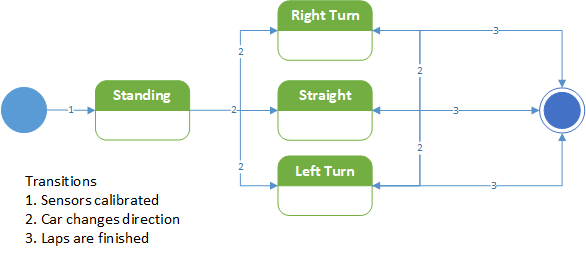
\includegraphics[scale=0.8]{Pictures/statemachine.png}
	\caption{Theoretical state machine}
	\label{statemachine}
\end{figure}

The flow the application is taking, is demonstrated in figure \ref{activitydiagram}. It can be seen that the user has two different options. First, a new session can be started, which is followed by positioning the car and calibrate the sensors. The other option is to review previous sessions. Therefore the user must select one of the stored data sets. When choosing a new session, the start of the race is triggered, when the car leaves the start. The race finish is triggered by pressing a button. The next step is the same for both decisions of the user. The data set, new or old, is taken and analysed. This is done to provide backward compatibility, when updates are rolled out. After the data has been processed, the report is created with tips for performance improvement.

\begin{figure}[H]
	\centering
	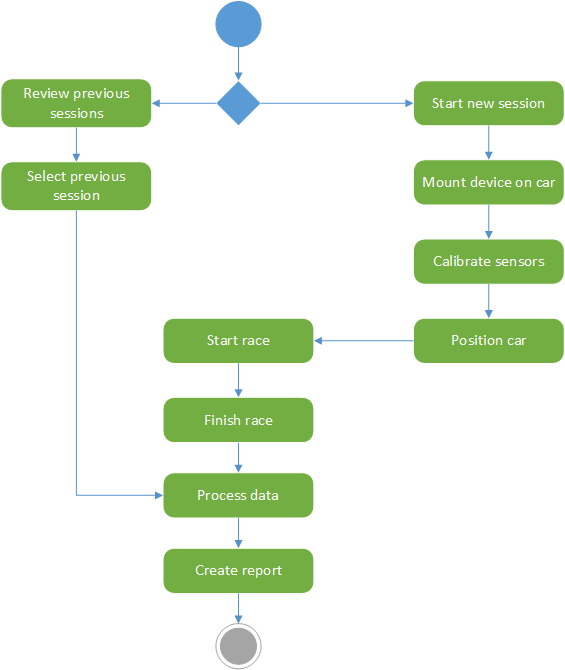
\includegraphics[scale=0.8]{Pictures/activitydiagram.png}
	\caption{Activity diagram of LapOps}
	\label{activitydiagram}
\end{figure}
\chapter{Mathematical Models of Identifying Sections}

\section{Data Analysis}
The following section describes the data used. To ensure that the data recorded via the accelerometer can be evaluated, modifications such as smoothing and noise filtering had to be made. These are described below. But first the used data model is shown.

\subsection{Data Model}
The used Model consists of four parameters:
\begin{itemize}
	\item \textbf{Round}: represents the current lap
	\item \textbf{Time Stamp}: represents the current time stamp for each step
	\item \textbf{X-Acceleration}: represents the force that indicates curves
	\item \textbf{Y-Acceleration}: represents the force that indicates the acceleration of the vehicle
\end{itemize}
The reason, why only the forces in x- and y-directions are used, is that the device lies flat on the vehicle. In this case the z-acceleration only indicates the force of gravity, which is not necessary for this work.\\
The round is not altered, therefore it will not be mentioned any further. 

For the initial data one entry containing the four parameters is taken every 10 milliseconds. Figure \ref{fig:origFor} shows the forces for one lap in the original data.

\begin{figure}[H]
	\centering
	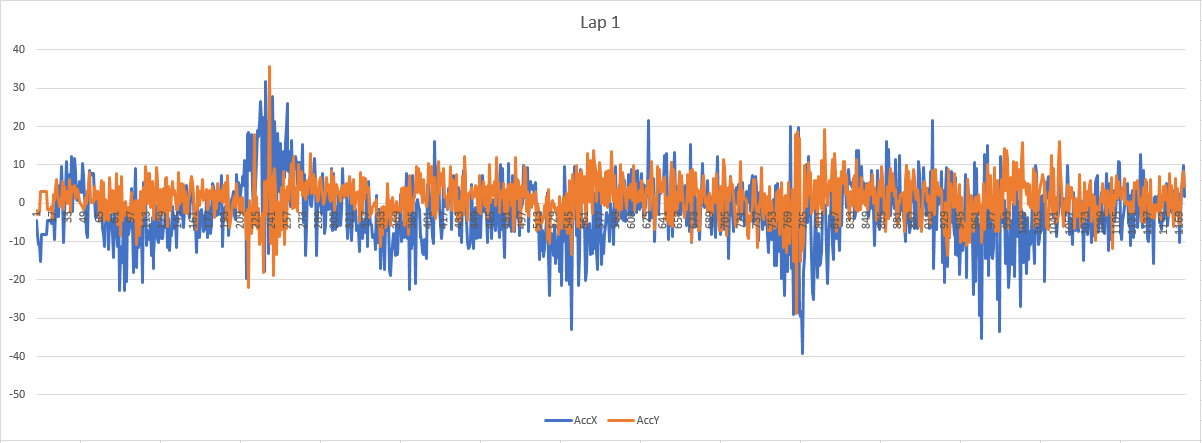
\includegraphics[scale= 0.42]{Pictures/originalForces.png}
	\caption{Visualization of the forces in the original data}
	\label{fig:origFor}
\end{figure}

This figure shows clearly that a analysis on base of the unfiltered data is simply impossible. Therefore as a first step data smoothing is used which is described in the following.

\subsection{Smoothing}
One problem that was identified is that there are to many measured points over time. So at first every four to five measured points were summed up and the average was used. This resulted in a better graph, which is shown in figure \ref{fig:smoFor}.

\begin{figure}[H]
	\centering
	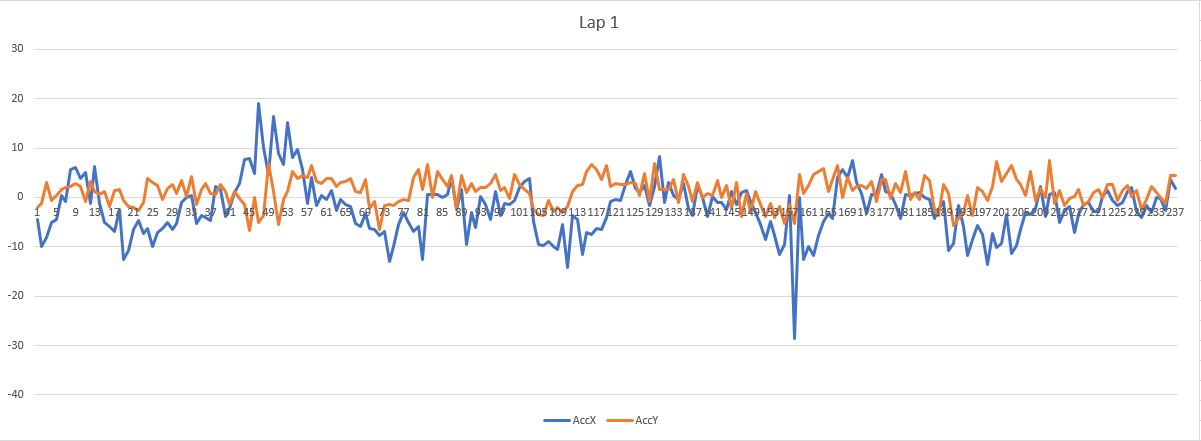
\includegraphics[scale= 0.45]{Pictures/smoothedForces.png}
	\caption{Visualization of the forces of the smoothed data}
	\label{fig:smoFor}
\end{figure}

In this figure it is possible for the human eye to distinguish between sections like left and right curves. But because of the noise, it would still be difficult for a computer. So a noise filter had to be used. It is described in the following section.

\subsection{Savitzky-Golay Filtering}
This filter is used to increase the signal-to-noise-ratio of a digital data set\cite{sg}. Therefore it would perfectly fit the requirement. It requires a data set consisting of $n$ points $(x,y)$ where x is an independent variable and y is the observed value. In this case $x$ is the time stamp, while $y$ is the force in x-/y- direction. In addition a set of $m$ convolution coefficients $C_i$ are needed which results in following equation:
\begin{equation*}
	Y_j = \sum_{i=-\frac{m-1}{2}}^{\frac{m-1}{2}}\dfrac{C_i\cdot y_{j+i}}{h},~~~~~~~ \dfrac{m-1}{2}\leq j \leq n-\dfrac{m-1}{2}
\end{equation*}
Because of the high sample rate in this project a relatively high value for $m=9$ was used. Therefore 9 convolution coefficients were used:
\begin{equation*}
	\begin{split}
	C_{-4} & = -21\\
	C_{-3} & = 14\\
	C_{-2} & = 39\\
	C_{-1} & = 54\\
	C_{0} & = 59   \\
	C_{1} & = 54     \\
	C_{2} & = 39     \\
	C_{3} & = 14     \\
	C_{4} & = -21    \\
	\end{split}
\end{equation*}
The sum of these coefficients is used for the normalisation $h=231$.

Applying this filter on the not smoothed original data results in a graph shown in figure \ref{fig:sgoriFor}.

\begin{figure}[H]
	\centering
	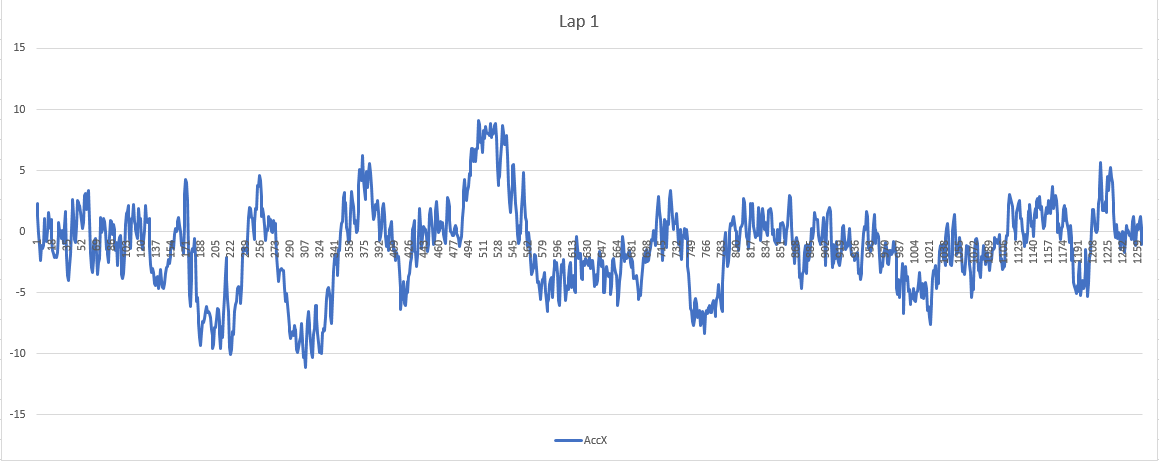
\includegraphics[scale= 0.45]{Pictures/sgoriForces.png}
	\caption{Visualization of the forces of the applied filter on the original data}
	\label{fig:sgoriFor}
\end{figure}

This proves, that a pre-smoothing might be needed to get a less noisy graph. Therefore figure \ref{fig:sgFor} shows the graph that is accomplished after applying both methods.

\begin{figure}[H]
	\centering
	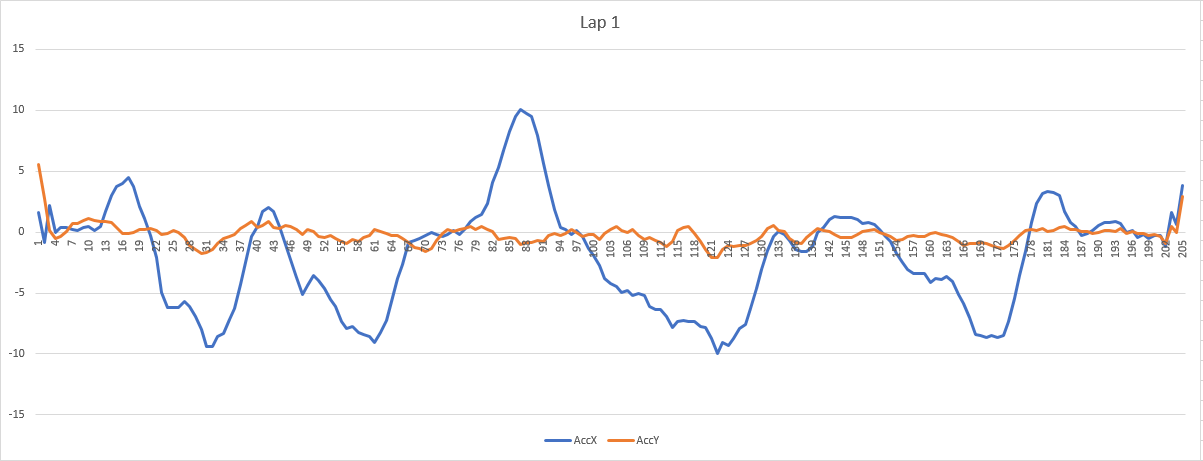
\includegraphics[scale= 0.45]{Pictures/sgForces.png}
	\caption{Visualization of the forces of the applied filter on the smoothed data}
	\label{fig:sgFor}
\end{figure}

With all this smoothing and filtering it is now possible for a computer to identify sections, which is described in the next section.

\newpage
\section{Section Identification}
The following section will describe the solution for the identification of sections. And is split into two parts. The first explains the rough identification of sections. These sections will then be given to a classification method that clearly identifies the type of section, be it a curve or a straight line. 

\subsection{Identification}
The identification is split into three parts that will be executed serial. After smoothing and filtering of the dataset. The x-axis acceleration values will be split into two groups. This split is happening with a singular x value representing a threshold. In the positive and negative acceleration range. A visual representation of the threshold can be seen in figure \ref{upperlowerBound}. in this case, the threshold is set to 3.5. All points below the lower bound and above the upper bound will be grouped inside a dataset, while all the points in between are grouped in another.
\begin{figure}[H]
	\centering
	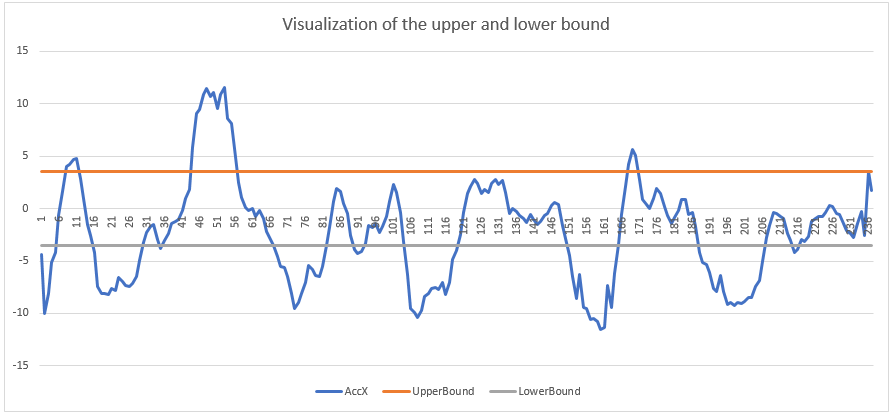
\includegraphics[scale= 0.6]{Pictures/upperandlowerbound.png}
	\caption{Visualization of the thresholds for the upper and lower dataset}
	\label{upperlowerBound}
\end{figure}
After separating the datasets with the threshold, the points above the threshold are considered as expected curves. Therefore it is cleaned in a second step. Because a curve cannot be created with only one point above the threshold, single points will be put back into the dataset in between the thresholds. The last step is grouping the points into sections. The points in between are created as new sections with ten points. A section, that is above the threshold will be created with the first point above and the last point above.

\subsection{Classification}

\section{Section Rating}
Because the focus of our project was the identification of sections, the section rating part contains a simple implementation. The core principle is determining the fastest lap and comparing the time footprint of the other sections to the sections of the fastest lap. Because in our model, a straight is following on a curve and vice versa, the following mappings are created. Figure \ref{StraightResultMapping} shows the mapping for a straight and the timestamp configurations while figure \ref{CurveResultMapping} shows the same for the curve. The green and red markings are showing, if the current lap is faster(green) or slower(red) on the current section than the fastest lap, that is chosen as reference.
\begin{figure}[H]
	\centering
	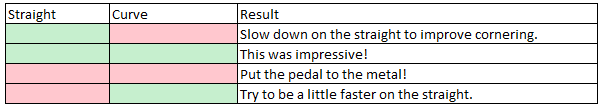
\includegraphics[scale= 0.9]{Pictures/StraightResultMapping.png}
	\caption{Mapping of the timestamps to the tips for a section, that is a straight}
	\label{StraightResultMapping}
\end{figure}

\begin{figure}[H]
	\centering
	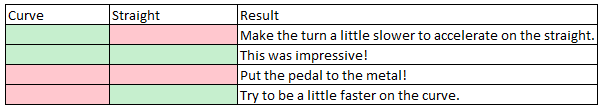
\includegraphics[scale= 0.9]{Pictures/CurveResultMapping.png}
	\caption{Mapping of the timestamps to the tips for a section, that is a curve}
	\label{CurveResultMapping}
\end{figure}

\chapter{LapOps Application}

\section{How to use it}

\section{Additional Information}
\chapter{Conclusion}
The project started with problems, since the data collected from driving a car was a lot different than data got by driving a RC-Car. The project had to adapt and focus on important objectives.

Data analysis and modification made it possible to reach a degree of reliability, that was not expected this high, since real world data is far from perfect and accidents happen, especially while racing.

The project has great further potential to be more robust, more precise and give better tips. By taking the remaining acceleration axis into account, the range of the tips could be increased as well as the section identification could be done even more robust by looking at more data. Another possible addition would be a neural network fed with training data to recognise racing patterns. Even real-time section identification could be possible that way. 


%---------------------------------------------------------------------
%--- Bibliography and appendices
%---------------------------------------------------------------------



		
\end{document}
